\documentclass[a4paper,12pt]{article}

\usepackage[slovene]{babel}
\usepackage[T1]{fontenc}
\usepackage[utf8]{inputenc}
\usepackage{amsmath,amssymb}
\usepackage{xcolor}
\usepackage[most]{tcolorbox}
\usepackage{titlesec}
\usepackage{pgfplots}
\usepackage{geometry}
\usepackage{enumitem}
\usepackage[colorlinks=true,linkcolor=blue,urlcolor=blue]{hyperref}

\pgfplotsset{
	compat=1.18,
	graphstyle/.style={
		width=0.62\textwidth,
		height=3.2cm,
		axis lines=middle,
		grid=major,
		grid style={gray!20},
		tick label style={font=\tiny},
		label style={font=\tiny},
		title style={font=\scriptsize},
		xlabel={$x$},
		ylabel={$y$},
		samples=100,
		clip=true
	}
}

\definecolor{bordotemno}{RGB}{101,8,34}
\definecolor{bordosvetlo}{RGB}{153,67,88}
\definecolor{rozasvetla}{RGB}{255,243,245}
\definecolor{zelenasvetla}{RGB}{78,139,82}
\newtcolorbox{vsebinskiokvir}{
	breakable,
	colback=rozasvetla,
	colframe=bordotemno,
	boxrule=1pt,
	arc=1.5mm,
	left=5mm,
	right=5mm,
	top=3mm,
	bottom=3mm,
	before skip=1.5ex,
	after skip=1.5ex
}
\titleformat{\section}{\normalfont\Large\bfseries\color{bordotemno}}{\thesection}{1em}{}
\titleformat{\subsection}{\normalfont\large\bfseries\color{bordosvetlo}}{\thesubsection}{1em}{}
\titleformat{\subsubsection}{\normalfont\normalsize\bfseries\color{bordosvetlo}}{\thesubsubsection}{1em}{}
\titlespacing*{\section}{0pt}{4.5ex plus 1ex minus .2ex}{2.5ex plus .3ex}
\titlespacing*{\subsection}{0pt}{3.5ex plus .8ex minus .2ex}{1.8ex plus .2ex}
\titlespacing*{\subsubsection}{0pt}{2.8ex plus .6ex minus .2ex}{1.3ex plus .2ex}

\newcommand{\vajaGraf}[6]{%
	\par\smallskip
	\begin{center}
		\begin{tikzpicture}
			\begin{axis}[graphstyle,title={#1},xmin=#2,xmax=#3,ymin=#4,ymax=#5]
				\addplot[blue,thick,domain=#2:#3]{#6};
			\end{axis}
		\end{tikzpicture}
	\end{center}
	\smallskip
}

\newcommand{\prazenKoordinatniSistem}[4]{%
	\par\smallskip
	\begin{center}
	\begin{tikzpicture}
	\begin{axis}[graphstyle,xmin=#1,xmax=#2,ymin=#3,ymax=#4]
	\end{axis}
	\end{tikzpicture}
	\end{center}
	\smallskip
}

\geometry{margin=2.4cm}
\setlist{itemsep=2pt,topsep=4pt}

\title{\textcolor{bordotemno}{Pregled snovi: funkcije}\\\large\textcolor{bordosvetlo}{Matematika, 2. letnik}}
\author{}
\date{}

\begin{document}

\maketitle
\newpage
{\hypersetup{linkcolor=zelenasvetla}\color{zelenasvetla}\tableofcontents}
\hypersetup{linkcolor=blue}
\newpage

\section{Učni načrt in cilji}

Pregled povzema tipične vsebine o funkcijah, ki se obravnavajo v 2. letniku srednje šole. Vrstni red in obseg posameznih tem se lahko med programi in učitelji nekoliko razlikujeta.

\begin{vsebinskiokvir}
\subsection*{Kaj naj bi znal/-a?}
Po obravnavi snovi naj bi znal/-a:
\begin{itemize}
	\item razložiti pojem funkcije ter določiti definicijsko območje in zalogo vrednosti;
	\item funkcijo predstaviti s predpisom, tabelo, grafom ali opisom;
	\item izračunati ničle, začetno vrednost in presečišča grafa z osema;
	\item iz grafa ali predpisa razbrati predznak, monotonost, omejenost in ekstreme;
	\item ugotoviti, ali je funkcija soda, liha ali periodična;
	\item prepoznati in raziskati potenčne funkcije ter njihove osnovne grafe;
	\item uporabiti lastnosti funkcij pri reševanju enačb, neenačb in besedilnih nalog.
\end{itemize}
\end{vsebinskiokvir}

\clearpage
\section{Pojem funkcije}

\begin{vsebinskiokvir}
Funkcija $f$ iz množice $D$ v množico $Z$ vsakemu elementu $x\in D$ priredi natanko en element $y\in Z$. Zapišemo
\[
	f\colon D\to Z,\qquad y=f(x).
\]
Množica $D$ je \emph{definicijsko območje} funkcije, množica vseh dejansko doseženih vrednosti $f(x)$ pa \emph{zaloga vrednosti} (označimo jo z $Z_f$). Vrednost $x$ imenujemo argument, vrednost $f(x)$ pa funkcijska vrednost.
\end{vsebinskiokvir}

\subsection{Kako funkcijo podamo?}
\begin{itemize}
	\item s predpisom, na primer $f(x)=2x-1$;
	\item s tabelo vrednosti;
	\item z grafom v koordinatnem sistemu;
	\item z besednim opisom ali diagramom prirejanja.
\end{itemize}

Graf funkcije je množica točk $(x,f(x))$. Navpična premica lahko graf funkcije seka največ enkrat: če ga seka večkrat, bi enemu argumentu pripadalo več funkcijskih vrednosti.

\subsection{Definicijsko območje}

Če ni drugače povedano, poiščemo največjo množico realnih števil, za katera je predpis smiseln. Pri tem preverimo predvsem:
\begin{itemize}
	\item imenovalec ulomka ne sme biti enak $0$;
	\item podkoren izraz pri sodem korenu mora biti nenegativen;
	\item izraz pod logaritmom mora biti pozitiven.
\end{itemize}
Primeri:
\[
	f(x)=\frac{1}{x-3}:\quad D_f=\mathbb{R}\setminus\{3\},\qquad
	g(x)=\sqrt{x+2}:\quad D_g=[-2,\infty).
\]

\clearpage
\section{Osnovni pojmi in odčitavanje grafa}
\begin{vsebinskiokvir}

\begin{itemize}
	\item \textbf{Ničla:} število $x_0$, za katero velja $f(x_0)=0$. Na grafu je to presečišče z osjo $x$.
	\item \textbf{Začetna vrednost:} $f(0)$, če je $0\in D_f$. Graf seka os $y$ v točki $(0,f(0))$.
	\item \textbf{Predznak:} določimo, kje je $f(x)>0$, $f(x)<0$ oziroma $f(x)=0$.
	\item \textbf{Presečišče grafov:} velja $f(x)=g(x)$; abscise presečišč so rešitve enačbe.
	\item \textbf{Vodoravna premica:} enačba $y=c$ seka graf pri tistih $x$, za katere je $f(x)=c$.
\end{itemize}

Pri skici grafa najprej določimo definicijsko območje, ničle, presečišče z osjo $y$, predznak in značilne lastnosti. Nato narišemo dovolj značilnih točk in upoštevamo obliko grafa.
\end{vsebinskiokvir}

\clearpage
\section{Lastnosti funkcij}

\subsection{Naraščanje in padanje}

Funkcija je na intervalu naraščajoča, če za $x_1<x_2$ velja $f(x_1)\leq f(x_2)$; strogo naraščajoča je, če velja stroga neenačba. Padajočo funkcijo opredelimo z obrnjenim vrstnim redom vrednosti. Monotonost lahko velja na celotnem definicijskem območju ali le na posameznih intervalih.

\subsection{Omejenost}

Funkcija je navzgor omejena, če obstaja število $M$, za katero je $f(x)\leq M$ za vsak $x\in D_f$. Navzdol omejena je, če obstaja $m$, da je $f(x)\geq m$. Omejena je, če je omejena navzgor in navzdol.

Primer: $f(x)=x^2$ je navzdol omejena z $0$, navzgor pa ni omejena. Funkcija $g(x)=\sin x$ je omejena, saj velja $-1\leq g(x)\leq 1$.

\subsection{Ekstremi}

Vrednost $f(a)$ je maksimum, če velja $f(x)\leq f(a)$ za vse $x\in D_f$; minimum določimo analogno. Lokalni ekstrem je največja ali najmanjša vrednost le v bližnji okolici točke. Ekstrem ni nujno dosežen: na primer $f(x)=x$ na intervalu $(0,1)$ nima minimuma niti maksimuma.

\subsection{Konveksnost in konkavnost}

Na intervalu je funkcija konveksna, če daljica med poljubnima točkama njenega grafa leži nad grafom ali na njem. Konkavna je, če daljica leži pod grafom ali na njem. Pri konveksni funkciji se nakloni sekantnih premic z leve proti desni ne zmanjšujejo; pri konkavni se ne povečujejo. Na primer, $f(x)=x^2$ je konveksna na $\mathbb{R}$, $g(x)=-x^2$ pa konkavna. Če so odvodi že obravnavani, lahko konveksnost na intervalu preverimo z $f''(x)\geq 0$, konkavnost pa z $f''(x)\leq 0$.

Prevoj je točka, v kateri se graf spremeni iz konveksnega v konkavnega ali obratno. Sama sprememba predznaka drugega odvoda je lahko dokaz prevoja, vendar je treba preveriti, da se konveksnost oziroma konkavnost na tej točki dejansko zamenja.

\subsection{Sode in lihe funkcije}

Definicijsko območje mora biti simetrično glede na $0$ (če je $x$ v območju, mora biti tudi $-x$). Nato preverimo:
\begin{align*}
	f(-x)=f(x)&\quad\Longrightarrow\quad \text{funkcija je soda},\\
	f(-x)=-f(x)&\quad\Longrightarrow\quad \text{funkcija je liha}.
\end{align*}
Graf sode funkcije je simetričen glede na os $y$, graf lihe funkcije pa glede na koordinatno izhodišče. Primeri: $x^2$ in $|x|$ sta sodi; $x^3$ in $\frac{1}{x}$ (na svojem območju) sta lihi. Funkcija je lahko tudi niti soda niti liha.

\subsection{Periodičnost}

Funkcija je periodična, če obstaja $T>0$, da za vsak $x$ iz definicijskega območja velja $f(x+T)=f(x)$ (kjer sta obe vrednosti določeni). Najmanjše tako pozitivno število je osnovna perioda. Funkciji $\sin x$ in $\cos x$ imata periodo $2\pi$.

\subsection{Injektivnost in inverzna funkcija}

Funkcija je injektivna, če različna argumenta vedno določita različni vrednosti. Graf prestane preizkus z vodoravno premico, če ga vsaka vodoravna premica seka največ enkrat. Injektivna funkcija ima obratno funkcijo na svoji zalogi vrednosti; vloga argumenta in vrednosti se zamenja. Pri funkciji $f(x)=2x+1$ je $f^{-1}(x)=\frac{x-1}{2}$.

\subsection{Učni načrt: lastnosti funkcij}

Pri tej temi dijak/-inja iz grafa in predpisa določi intervale naraščanja in padanja, predznak, omejenost ter ekstreme; preveri sodost, lihost in periodičnost; prepozna konveksnost, konkavnost in morebitni prevoj. Lastnosti zna utemeljiti s simetrijo grafa, primerjavo funkcijskih vrednosti ali ustrezno metodo, ki je bila obravnavana pri pouku.

\subsection{Vaje v slogu maturitetnih nalog: lastnosti}

Naslednje naloge so izvirne vaje za ponavljanje in niso prepisana uradna vprašanja iz mature 2024.
\begin{enumerate}
	\item Za $f(x)=|x-2|$ določi ničlo, zalogo vrednosti, intervale monotonosti in preveri, ali je funkcija soda ali liha.
	\item Skiciraj $g(x)=\frac{1}{x^2+1}$ ter iz grafa oziroma predpisa določi območje, zalogo vrednosti, omejenost in sodost.
	\item Opiši konveksnost funkcije $h(x)=x^2-4x+1$ in določi njeno najmanjšo vrednost.
\end{enumerate}

\clearpage
\section{Potence in potenčne funkcije}
\begin{vsebinskiokvir}

Potenčna funkcija ima predpis
\[
	f(x)=x^n,
\]
kjer je eksponent $n$ izbrano realno ali celo število. Oblika grafa in definicijsko območje sta odvisna od eksponenta.
\end{vsebinskiokvir}

\subsection{Naravni eksponent}

Za $n\in\mathbb{N}$:
\begin{itemize}
	\item če je $n$ sod, je $x^n\geq 0$, funkcija je soda; pada na $(-\infty,0]$ in narašča na $[0,\infty)$; minimum je $0$;
	\item če je $n$ lih, je funkcija liha in strogo narašča na $\mathbb{R}$; njena zaloga vrednosti je $\mathbb{R}$.
\end{itemize}
V obeh primerih je $D_f=\mathbb{R}$. Primeri osnovnih oblik sta parabolični graf $y=x^2$ in kubični graf $y=x^3$.

\subsection{Negativni celoštevilski eksponent}

Za $n\in\mathbb{N}$ velja
\[
	x^{-n}=\frac{1}{x^n},\qquad D_f=\mathbb{R}\setminus\{0\}.
\]
Graf ne seka osi $x$ in $y$. Premici $x=0$ in $y=0$ sta asimptoti. Funkcija $x^{-n}$ je soda za sod $n$ in liha za lih $n$. Na primer, $y=\frac1{x^2}$ je pozitivna in soda, $y=\frac1x$ pa liha.

\subsection{Koren in racionalni eksponent}

Za pozitivni celi števili $m,n$ in ustrezno določeno realno potenco velja
\[
	x^{m/n}=\sqrt[n]{x^m}.
\]
Pri sodem korenu mora biti korenjenec nenegativen; pri lihih korenih so dovoljene tudi negativne vrednosti. Vedno upoštevamo tudi, ali je potenca v imenovalcu ulomka. Primeri: $\sqrt{x}$ ima območje $[0,\infty)$, medtem ko je kubični koren $\sqrt[3]{x}$ določen za vsak $x\in\mathbb{R}$.

\subsection{Premiki in raztegi grafov}

Iz grafa $y=f(x)$ dobimo:
\begin{itemize}
	\item $y=f(x)+k$: premik za $k$ navpično;
	\item $y=f(x-h)$: premik za $h$ vodoravno v desno;
	\item $y=a f(x)$: navpični razteg ali skrčitev; pri $a<0$ še zrcaljenje čez os $x$;
	\item $y=f(-x)$: zrcaljenje čez os $y$.
\end{itemize}
Pri vodoravnih spremembah predznak v oklepaju pogosto deluje nasprotno od pričakovanja: $f(x-3)$ je premik v desno za $3$.

\subsection{Učni načrt: potenčna funkcija}

Dijak/-inja primerja grafe $x^n$ za sode in lihe naravne eksponente ter grafe $x^{-n}$ za negativne cele eksponente. Za izbrano potenčno funkcijo določi definicijsko območje, zalogo vrednosti, ničle, simetrijo, monotonost, omejenost in asimptote, kadar obstajajo. Zna uporabiti potence in premike grafa pri reševanju enačb ter pri preprostih modelih.

\subsection{Vaje v slogu maturitetnih nalog: potenčna funkcija}

To so izvirne naloge za pripravo na preverjanje znanja, ne uradna vprašanja iz mature 2024.
\begin{enumerate}
	\item Za $f(x)=x^5$ in $g(x)=x^4$ primerjaj definicijski območji, zalogi vrednosti, simetriji in monotonost.
	\item Nariši $h(x)=\frac{1}{x^2}$ in navedi njeni asimptoti. Reši neenačbo $h(x)>1$.
	\item Graf $y=x^3$ premakni za $2$ enoti levo in $1$ enoto navzdol. Zapiši predpis nove funkcije in preveri njeno lihost.
\end{enumerate}

\clearpage
\section{Korenska funkcija}
\begin{vsebinskiokvir}

Korenska funkcija je funkcija oblike
\[
	f(x)=\sqrt[n]{x},
\]
kjer je $n$ naravno število. Pri sodem $n$ mora biti $x\geq 0$, zato je $D_f=[0,\infty)$; pri lihem $n$ je $D_f=\mathbb{R}$. Pri sodem korenu so tudi vrednosti nenegativne. Pri lihem korenu je zaloga vrednosti $\mathbb{R}$.
\end{vsebinskiokvir}

Korenska funkcija je inverzna funkcija ustrezne potenčne funkcije na intervalu, kjer je ta injektivna. 
Tako je $y=\sqrt{x}$ inverzna funkcija funkcije $y=x^2$, 
če slednjo omejimo na $[0,\infty)$; grafa sta zrcalni sliki glede na premico $y=x$. 
Funkcija $y=\sqrt{x}$ je naraščajoča, njena ničla je $0$, graf pa se začne v koordinatnem izhodišču. 
Funkcija $y=\sqrt[3]{x}$ je liha in strogo naraščajoča na $\mathbb{R}$.

Pri določanju območja sestavljene korenske funkcije zahtevamo, da je izraz pod sodim korenom nenegativen. Na primer,
\[
	f(x)=\sqrt{3x-6}\quad\Longrightarrow\quad 3x-6\geq0\quad\Longrightarrow\quad D_f=[2,\infty).
\]

\subsection{Učni načrt: korenska funkcija}

Dijak/-inja določi definicijsko območje korenske funkcije, razlikuje med sodim in lihim korenskim eksponentom, nariše osnovni graf ter opiše njegovo monotonost in zalogo vrednosti. Razume povezavo med korensko in potenčno funkcijo ter zna reševati enačbe in preproste besedilne naloge s koreni.

\subsection{Vaje v slogu maturitetnih nalog: korenska funkcija}

Naloge so pripravljalne in izvirne; niso uradna vprašanja iz mature 2024.
\begin{enumerate}
	\item Določi definicijsko območje in ničlo funkcije $f(x)=\sqrt{5-2x}$.
	\item Reši enačbo $\sqrt{x+1}=3$ in preveri dobljeno rešitev v začetni enačbi.
	\item Skiciraj $y=\sqrt[3]{x}$ ter ga primerjaj z grafom $y=x^3$.
\end{enumerate}

\clearpage
\section{Nekaj pomembnih družin funkcij}
\begin{vsebinskiokvir}

\begin{itemize}
	\item \textbf{Linearna funkcija} $f(x)=kx+n$: graf je premica; $k$ je smerni koeficient, $n=f(0)$.
	\item \textbf{Kvadratna funkcija} $f(x)=ax^2+bx+c$, $a\ne0$: graf je parabola; njena os simetrije je $x=-\frac{b}{2a}$.
	\item \textbf{Polinomska funkcija}: vsota členov oblike $a_kx^k$; definirana je za vsa realna števila.
	\item \textbf{Racionalna funkcija}: količnik polinomov; iz območja izločimo ničle imenovalca.
	\item \textbf{Eksponentna funkcija} $a^x$, kjer $a>0$ in $a\ne1$: območje vrednosti je $(0,\infty)$; narašča za $a>1$ in pada za $0<a<1$.
	\item \textbf{Logaritemska funkcija} $\log_a x$: obratna je eksponentni funkciji $a^x$; določena je za $x>0$.
\end{itemize}
\end{vsebinskiokvir}

\clearpage
\section{Postopek raziskovanja funkcije}

Pri nalogi o funkciji si pomagamo z naslednjim seznamom:
\begin{enumerate}
	\item Določi definicijsko območje $D_f$.
	\item Izračunaj ničle in začetno vrednost, če obstaja.
	\item Preveri simetrijo: izračunaj oziroma primerjaj $f(-x)$ in $f(x)$.
	\item Ugotovi predznak in intervale naraščanja/padanja.
	\item Poišči omejenost in ekstreme; po potrebi preveri periodičnost.
	\item Določi značilne točke, nariši graf in iz njega odčitaj zalogo vrednosti.
\end{enumerate}
V praksi lastnosti pogosto odčitamo z grafa, v algebrskih nalogah pa jih utemeljimo s predpisom. Pri risanju je pomembno, da je vsaka točka grafa oblike $(x,f(x))$.

\clearpage
\section{Predlog zaporedja učnih ur}

Spodnji načrt je predlog za 17 šolskih ur; učitelj/-ica lahko vrstni red in zahtevnost prilagodi programu in predznanju razreda. Pri maturitetno zasnovanih nalogah v tem gradivu gre za izvirne vaje, ne za prepis uradnih vprašanj iz leta 2024.

\subsection{1. ura: Ponovitev snovi o funkcijah}
Ponovimo preslikavo, definicijsko območje, zalogo vrednosti, ničle in načine podajanja funkcije. Dijaki iz predpisa sestavijo tabelo vrednosti in narišejo preprost graf. Predlagana vaja: za $f(x)=2x-1$ določi $f(-1)$, $f(0)$, ničlo in presečišči z osema.

\subsection{2. ura: Naraščanje, padanje, predznak funkcije}
Monotonost in predznak odčitamo z grafa ter preverimo na preprostih predpisih. Predlagana vaja: za $f(x)=(x-1)(x+2)$ določi ničle in intervale, na katerih je funkcija pozitivna oziroma negativna.

\subsection{3. ura: Omejenost, sodost, lihost}
Razlikujemo omejenost od doseganja ekstremov ter uporabimo preizkusa $f(-x)=f(x)$ in $f(-x)=-f(x)$. Predlagana vaja: razvrsti $x^2$, $x^3$, $\frac1x$ in $x+1$ glede na sodost oziroma lihost ter utemelji.

\subsection{4. ura: Konveksnost, konkavnost}
Konveksnost in konkavnost prepoznamo po legi grafa glede na sekante; pogovorimo se tudi o prevoju. Predlagana vaja: primerjaj grafa $x^2$ in $-x^2$ ter opiši njuno ukrivljenost.

\subsection{5. ura: Vaje}
Utrdimo kombinirano raziskovanje funkcij: območje, ničle, predznak, monotonost, simetrijo, omejenost in skico. Dijaki v parih pripravijo celotno rešitev za eno izmed funkcij iz prejšnjih ur.

\subsection{6. ura: Transformacije na ravnini}
Spoznamo navpične premike in raztege ter zrcaljenje grafa. Predlagana vaja: iz grafa $y=x^2$ skiciraj $y=2x^2+1$.

\subsection{7. ura: Transformacije na ravnini}
Obravnavamo vodoravne premike in zrcaljenje čez os $y$ ter pazimo na predznak v argumentu. Predlagana vaja: skiciraj $y=(x-2)^2$ in $y=f(-x)$ za $f(x)=x^2+1$.

\subsection{8. ura: Transformacije na ravnini -- vaje}
Kombiniramo premike, raztege in zrcaljenja. Predlagana vaja: opiši transformacije iz $y=x^2$ v $y=-\frac12(x+1)^2+3$ ter določi vrh in zalogo vrednosti.

\subsection{9. ura: Inverzna funkcija}
Ponavljamo injektivnost, zamenjamo vlogi $x$ in $y$ ter rešimo enačbo za novo odvisno spremenljivko. Predlagana vaja: določi inverz funkcije $f(x)=3x-6$ ter preveri kompoziciji $f^{-1}(f(x))$ in $f(f^{-1}(x))$.

\subsection{10. ura: Dodatna ura}
Ura je namenjena odpravljanju težav, dodatnim razlagam ali razširitvi vsebin glede na potrebe razreda. Možne teme: branje zahtevnejših grafov, sestavljene funkcije ali priprava na preverjanje.

\subsection{11. ura: Potenčna funkcija z naravnim eksponentom}
Primerjamo potence s sodim in lihim eksponentom ter njihove grafe. Predlagana vaja: za $x^4$ in $x^5$ določi simetrijo, monotonost, ničle in zalogo vrednosti.

\subsection{12. ura: Vaje}
Ponavljamo potenčne funkcije z naravnim eksponentom, skiciranje in reševanje enačb. Predlagana vaja: reši $x^4=16$ in $x^5=-32$ ter rešitve preveri.

\subsection{13. ura: Potenčna funkcija z negativnim celim eksponentom}
Obravnavamo $x^{-n}=1/x^n$, izločeno vrednost $0$, simetrijo in asimptote. Predlagana vaja: za $1/x^2$ in $1/x^3$ primerjaj predznak, simetrijo in obnašanje v bližini $0$.

\subsection{14. ura: Vaje}
Utrdimo risanje in raziskovanje potenčnih funkcij z negativnim eksponentom. Predlagana vaja: reši $1/x^2=4$ in neenačbo $1/x^2<1$ ob upoštevanju definicijskega območja.

\subsection{15. ura: Korenska funkcija}
Povežemo korenske in potenčne funkcije ter določamo pogoje podkorenih izrazov. Predlagana vaja: določi območje $\sqrt{2x+4}$ in skiciraj $y=\sqrt{x-1}$.

\subsection{16. ura: Vaje}
Rešujemo enačbe s koreni, preverjamo rešitve in raziskujemo grafe. Predlagana vaja: reši $\sqrt{2x-1}=3$ ter preveri pogoj za obstoj in rešitev.

\subsection{17. ura: Modeliranje s potenčno in korensko funkcijo}
Iz besedilnega opisa izberemo spremenljivki, sestavimo model in razložimo njegove omejitve. Predlagana dejavnost: če je ploščina kvadrata $P$, zapiši dolžino stranice kot funkcijo $a(P)=\sqrt{P}$, določi smiselno območje in interpretiraj rezultat.

\clearpage
\section{Naloge za utrjevanje}

Naloge najprej reši brez vpogleda v rešitve. Pri nalogah 6, 7, 9 in 10 so prazni koordinatni sistemi za tvoje skice; grafe nariši sam/-a.
\begin{enumerate}[itemsep=2.2cm,topsep=0.8em]
	\item Za $f(x)=2x-3$ izračunaj $f(4)$, določi ničlo in začetno vrednost.
	\vajaGraf{Premica $y=2x-3$}{-2}{4}{-6}{6}{2*x-3}
	\item Raziskuj $g(x)=x^2-4$: določi območje, ničle, zalogo vrednosti, simetrijo, monotonost in minimum.
	\vajaGraf{Parabola $y=x^2-4$}{-3}{3}{-5}{5}{x^2-4}
	\item Za $h(x)=x^3$ ugotovi, ali je soda ali liha, določi monotonost in povej, ali je omejena.
	\vajaGraf{Kubična funkcija $y=x^3$}{-2}{2}{-8}{8}{x^3}
	\item Za $p(x)=\frac{1}{x-2}$ določi definicijsko območje, ničle, zalogo vrednosti in asimptote. Ali je funkcija omejena?
	\begin{center}
	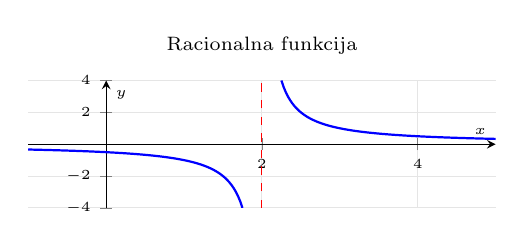
\begin{tikzpicture}
	\begin{axis}[graphstyle,title={Racionalna funkcija},xmin=-1,xmax=5,ymin=-4,ymax=4]
	\addplot[blue,thick,domain=-1:1.75]{1/(x-2)};
	\addplot[blue,thick,domain=2.25:5]{1/(x-2)};
	\addplot[red,dashed,domain=-4:4,samples=2] ({2},{x});
	\end{axis}
	\end{tikzpicture}
	\end{center}
	\item Za $q(x)=x^4-5x^2$ določi definicijsko območje, simetrijo, ničle in predznak.
	\vajaGraf{Soda funkcija $y=x^4-5x^2$}{-2.5}{2.5}{-7}{2}{x^4-5*x^2}
	\item Zapiši funkcijo, katere graf dobimo iz $y=x^2$ s premikom za $3$ enote desno in $2$ enoti navzgor. Določi njeno najmanjšo vrednost.
	\prazenKoordinatniSistem{-1}{7}{-2}{12}
	\item Določi definicijsko območje funkcij $r(x)=\sqrt{2x-6}$ in $s(x)=\frac{x+1}{x^2-9}$.
	\prazenKoordinatniSistem{0}{8}{0}{4}
	\prazenKoordinatniSistem{-5}{5}{-3}{3}
	\item Ugotovi, ali je $t(x)=x^2+2x$ soda, liha ali niti soda niti liha. Utemelji z izračunom $t(-x)$.
	\item Premica skozi točki $(0,2)$ in $(3,8)$ je graf linearne funkcije. Zapiši njen predpis in določi ničlo.
	\prazenKoordinatniSistem{-3}{3}{-4}{9}
	\item Skiciraj grafa $y=x^2$ in $y=(x-1)^2-2$. Opiši, kako sta povezana.
	\prazenKoordinatniSistem{-2}{4}{-4}{10}
\end{enumerate}

\clearpage
\subsection{Kratke rešitve}
\begin{enumerate}
	\item $f(4)=5$; ničla je $x=\frac32$; $f(0)=-3$.
	\item $D_g=\mathbb{R}$; ničle $-2,2$; $Z_g=[-4,\infty)$; soda; pada na $(-\infty,0]$, narašča na $[0,\infty)$; minimum $-4$ pri $x=0$.
	\item Liha; strogo narašča na $\mathbb{R}$; ni omejena ne navzgor ne navzdol.
	\item $D_p=\mathbb{R}\setminus\{2\}$; nima ničel; $Z_p=\mathbb{R}\setminus\{0\}$; asimptoti sta $x=2$ in $y=0$; ni omejena.
	\item $D_q=\mathbb{R}$; soda; ničle $x=0$ in $x=\pm\sqrt5$. Ker je $q(x)=x^2(x^2-5)$, je negativna za $0<|x|<\sqrt5$ in pozitivna za $|x|>\sqrt5$.
	\item $f(x)=(x-3)^2+2$; najmanjša vrednost je $2$.
	\item $D_r=[3,\infty)$; $D_s=\mathbb{R}\setminus\{-3,3\}$.
	\item $t(-x)=x^2-2x$; to ni enako niti $t(x)$ niti $-t(x)$, zato funkcija ni soda in ni liha.
	\item Smerni koeficient je $2$, zato je $f(x)=2x+2$; ničla je $x=-1$.
	\item Drugi graf je prvi premaknjen za $1$ v desno in za $2$ navzdol; vrh je $(1,-2)$, minimum pa $-2$.
\end{enumerate}

\end{document}
